\chapter{Companding - Redundancy Reduction}
\label{ch:part1}

\section{Companding}
I dette afsnit vil vi gennemgå begrebet `companding`, som en er sammentrækning af `compresseion`og `expansion`. 

Companding er i korte træk en metode til begrænse redundans i talesignaler. Dette gøres ved at transformere talens normale Laplacian distribuerede pdf, om til en mere rektangulær pdf, for derefter kunne kode signalet med en konstant-længde kode. Hos modtageren gendannes signalet til dets oprindelige form. Generelt vinder man 4 bits/sample ved companding, og kan altså ved 8 bit/sample, få et signal der har samme kvalitet som et signal med 12 bit/sample. 

\begin{figure}[!ht]
	\centering
	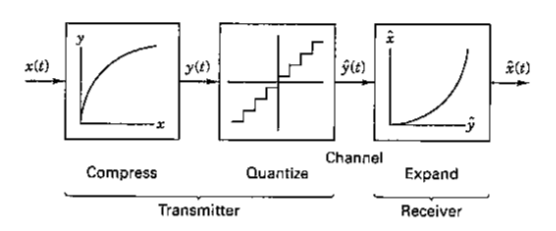
\includegraphics[width=0.8\textwidth]{resources/part1_compand_quant_expand}
 	\caption{Blokdiagram over companding (fra CampusNet-note om Source Coding)}
 	\label{fig:part1_1}
\end{figure}

I stedet for at bruge companding, kunne man benytte len non-uniform quantizer. Dette ville teoretisk have samme effekt.

Signalers kvalitet kan objektiv set beskrives ved hjælp af `Signal to Quantization Noise Ratio`, som er altså er et forhold mellem signalets samlede størrelse, og størelsen af den quantiserede signal. 



\section{Compression}
Formålet med compression-delen er, at gøre pdf-en mere rektangulær. Til dette findes forskellige standarder, bl.a. $\mu$-law compression, som er standarden i USA. Input-output karakteristikken for en $\mu$-law compressor er givet i ligning \ref{eq:part1_1}.

\begin{equation}\label{eq:part1_1}
	y = \frac{ln(1 + \mu|s|)}{ln(1+\mu)} sgn(s); \text{   } |s| \leq 1, |y| \leq 1
\end{equation}



\section{Expanding}
Den omvendte process kaldes expanding, og er simpelthen den inverse relation (ligning \ref{eq:part1_2}).

\begin{equation}\label{eq:part1_2}
	|s| = \frac{(1 + \mu)^|y| - 1}{\mu}; \text{   } |y| \leq 1, |s| \leq 1
\end{equation}



\section{Signal Quantization Noise Ratio - SQNR}
Når et signal quantiseres, opstår der en forskel mellem input-signalet og output-signalet. Denne forskel kaldes for `quantization error`, Hvis $s_q[n]$ er det quantiserede signal, og $s[n]$ er det originale signale, så kan quantiserings-error'en beskrives ved hjælp af ligning \ref{eq:part1_3}.

\begin{equation}\label{eq:part1_3}
	q[n] = s_q[n] - s[n]
\end{equation}

For at illustrere quantization-error, kigger vi på quantiseringen af en sinus. Figur \ref{fig:part1_2} viser en 1 Hz sinus (blå), og det 4-bit quantiserede signal (blå). 

\begin{figure}[!ht]
 	\centering
 	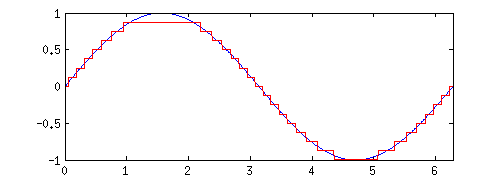
\includegraphics[width=0.8\textwidth]{resources/part1_sine_quant}
 	\caption{Sinus - quantiseret med 4-bit}
 	\label{fig:part1_2}
\end{figure}

 På figuren ses det tydeligt at fejlen er størst i toppen og bunden af sinus'en. Selve fejlen kan ses på figur \ref{fig:part1_3}.

\begin{figure}[!ht]
 	\centering
 	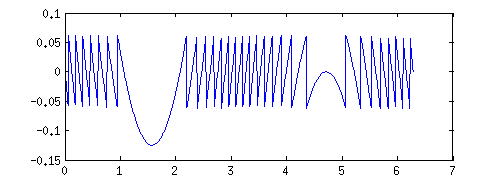
\includegraphics[width=0.8\textwidth]{resources/part1_sine_quant_error}
 	\caption{Sinus quantization error}
 	\label{fig:part1_3}
\end{figure}

For at objektivt beskrive kvaliteten af en quantisering, kigger man på forholdet mellem energien i det originale signal, og energien i quantization error'en. Ligning \ref{eq:part1_4} viser formlen for SQNR.

\begin{equation}\label{eq:part1_4}
	\text{SQNR} = 10 \cdot log_{10} \left( \frac{\sigma^2}{D} \right)
\end{equation}

Hvor $\sigma^2$ er mean square value af input-signalet (zero-mean), og $D$ er mean square af quantization error.

\subsection{SQNR for et sinus-signal}

For et sinus-signalet kan vi udlede en formel for SQNR, udfra et givent antal bits. Vi antager at amplituden for signalet er $V/2$. Først udregnes $\sigma^2$ og $D$ i ligning \ref{eq:part1_5}.

\begin{equation}\label{eq:part1_5}
	\begin{aligned}
	\sigma^2 &= \frac{1}{2\pi} \int_0^{2\pi} \left( \frac{V}{2} sin(x) \right) dx = \frac{V^2}{8} \\
	D &= \frac{\left( \frac{V}{L} \right)^2}{12} = \frac{V^2}{12 L^2}
	\end{aligned}
\end{equation}

Herefter kan vi udlede udtrykket for SQNR i ligning \ref{eq:part1_6}.

\begin{equation}\label{eq:part1_6}
	\text{SQNR} = 10 \cdot log_{10} \left( \frac{\frac{V^2}{8}}{\frac{V^2}{12 L^2}} \right) = 10 \cdot log_{10} \left( \frac{3}{2} L^2 \right) = 20 \cdot log_{10} (L) + 1.76\ dB
\end{equation}

Hvis $L = 2^B$ (B-bits quantizer), kan ligning \ref{eq:part1_6} reduceres endnu mere (ligning \ref{eq:part1_7}).

\begin{equation}\label{eq:part1_7}
	\text{SQNR} = 20 \cdot log_{10}(2^B) + 1.76\ dB = (6.02 B + 1.76)\ dB
\end{equation}

\section{Analyse af optaget tale}

I dette afsnit vil vi bruge de førnævnte begreber til at analysere et stykke optaget tale. Filen med talen, oak.wav, er samplet med 8 kHz, med 16 bits/sample. Vi lægger ud med at quantize signalet med 12 bit, for at have en reference, som vi kan sammenligne signalet med efter companding. 

 \begin{figure}[!ht]
 	\centering
 	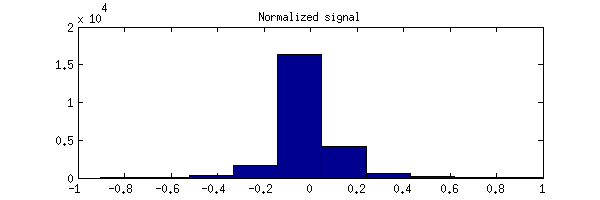
\includegraphics[width=0.8\textwidth]{resources/part1_original}
 	\caption{Pdf for originalt quantized signal}
 	\label{fig:part1_4}
 \end{figure}

 Det originale signal er quantized med 12 bits, hvilket giver en pdf som ses på figur \ref{fig:part1_4}. Som det kan ses er pdf'en ikke særlig rektangulær, men minder derimod meget om en Laplacian distribution. I MATLAB kan vi udregne SQNR til at være $59.22\ dB$. Vores mål med companding er altså at opnå en større SQNR med samme antal bits, eller opnå samme SQNR, med lavere antal bits. 

\subsection{Compression}
Først komprimeres signalet for at opnå en mere rektangulær pdf. Figur \ref{fig:part1_5} viser pdf'en, efter at signalet er blevet compressed med mu-law compression. Det er tydeligt at signalet ikke er blevet fuldstændig rektangulært, men dog meget mere rektangulært end det originale signals pdf. Det er nu på tide at lave en quantization af signalet, i første omgang med 12 bits som referencen.

\begin{figure}[!ht]
	\centering
	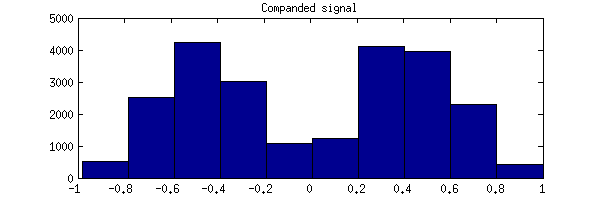
\includegraphics[width=0.8\textwidth]{resources/part1_compressed}
 	\caption{Pdf for compressed signal}
 	\label{fig:part1_5}
\end{figure}

\subsection{Expanding}
Signalet er nu først blevet compressed, og herefter quantized. Det er dermed på tide at expande signalet tilbage til dets oprindelige form. Figur \ref{fig:part1_6} viser pdf'en for signalet efter at det er blevet expanded. I MATLAB udregnes signals SQNR til at være $70.9\ dB$ - SQNR er altså blevet betydelig større. Det er altså muligt at opnå et signal med væsentlig mindre støj, ved hjælp af samme antal bits.

\begin{figure}[!ht]
	\centering
	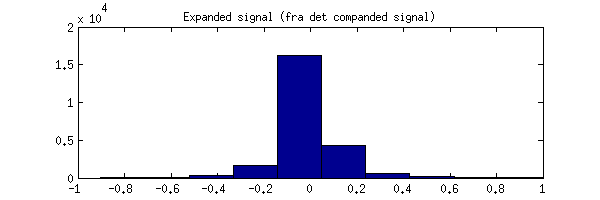
\includegraphics[width=0.8\textwidth]{resources/part1_expanded}
 	\caption{Pdf for expanded signal}
 	\label{fig:part1_6}
\end{figure}

\subsection{Færre bits - samme kvalitet}
Det kunne nu være interessant at undersøge, hvor få bits vi behøver at bruge for at opnå den samme kvalitet som i referencen. 

MATLAB afslører, at ved en quantization ved 10 bits, får vi en SQNR på $58\ dB$. Vi kan altså bruge 2 bits mindre, og stadig opnå tilnærmelsesvis samme kvalitet.

\subsection{Entropy}

Ved hjælp af MATLAB's entropy funktion, kan vi udregne entropien for signalerne.




